\documentclass[11pt,twoside,romanian]{extbook}
\usepackage[T1]{fontenc}
\usepackage[utf8]{inputenc}
\usepackage{color}
\usepackage{comment}
\usepackage{times}
\usepackage[margin=1in]{geometry}
\usepackage{fancyhdr}
\usepackage{lscape}
\usepackage{float}
\usepackage{listings}
\usepackage{babel}
\usepackage{amsmath}
\usepackage{amssymb,amsfonts,textcomp}
\usepackage{array}
\usepackage{hhline}
\usepackage[pdftex]{graphicx}
\usepackage[pdftitle={ANEXE - Sistemul de acces la date}, pdfauthor={RODA}, colorlinks=true, linkcolor=blue]{hyperref}

%\hypersetup{pdftex, colorlinks=true, linkcolor=blue, citecolor=blue, filecolor=blue, urlcolor=blue, pdftitle=, pdfauthor=, pdfsubject=, pdfkeywords=}
\pagestyle{fancy}
\DeclareGraphicsExtensions{.png,.gif,.jpg,.pdf}
\addto\captionsromanian{\renewcommand{\chaptername}{Anexa}}

\begin{document}

\pagenumbering{arabic} 
\cfoot{\tiny{RODA}\tiny}
\fancyhead[LE,RO]{ANEXE - \leftmark}
\fancyhead[RE,LO]{\thepage}

%TODO Change it every time !
\title{ANEXA 1.\\
Faza nr. III 
cu titlul:\\
``Dezvoltarea software, pachet 2: biblioteci nucleu, sistem template, autentificare. Raport privind modernizarea dot\u{a}rilor''
}

\author{RODA -- Arhiva Rom\^{a}n\u{a} de Date Sociale}

\date{ }

\maketitle

\newpage
\thispagestyle{plain}
\tableofcontents{}
\setcounter{page}{1}

\chapter{Componente ale aplicatiei}
\section{Arhitectura generala a aplicatiei Spring}

Intr-o aplicatie web moderna, exista o separare clara intre layers /
nivele. O aplicatie ce utilizeaza Spring MVC (Spring 3.2.x) va avea cel putin
cele 3 nivele specifice unei aplicatii MVC, respectiv Model, Views, Controllers; 
suplimentar, aplicatia RODA are definit un nivel de servicii, 
care permite izolarea modelului fata de controllere si specificarea de drepturi de acces personalizate (prin ACL). 
Exista servicii disponibile expuse aplicatiei ca JavaBeans, precum cele pentru: 
indexare si cautare; file-repository; 
integrarea unui motor statistic; 
executia asincrona sau programata de task-uri etc.

%TODO Diagrame UML componente si clase ???

Pentru dezvoltare se utilizeaza IDE-ul STS
\footnote{\url{http://www.springsource.org/sts}}.
Initial, in primele etape ale proiectului a fost utilizt si Spring Roo
\footnote{\url{http://www.springsource.org/spring-roo}}
(care permite sincronizarea schema BD - model, sincronizarea model-controllers-views si generarea de
interfete web tip CRUD, adaugarea de servicii si componente, structurarea proiectului si generarea de configuratii).

Pentru mentinerea sincronizarii intre schema bazei de date si modelul generat
in Java, s-a utilizat in primele etape ale proiectului metoda \emph{Forward-Engineering}: 
pornindu-se de la un editor grafic al schemei bazei de date (DbWrench 2), %TODO URL ???
se obtine scriptul de creare a bazei de date, 
care este post-procesat si care este apoi folosit de Spring Roo pentru
actualizarea modelului domeniului.

\subsection{Modelul domeniului}
Pentru specificarea modelului domeniului - specific aplicatiei RODA, 
am utilizat specificatia JPA 2.0 (Java Persistence API).

Astfel, pornind de la schema bazei de date prezentate in raportul etapei 1 (ce
a suferit unele modificari pentru a se apropia de standardul DDI Codebook si
de Spring Security), sunt definite \emph{entitati} in sensul JPA 2.0; 
aceste Java Beans (ce compun pachetul \emph{ro.roda.domain}) 
sunt independente (fara relatii de mostenire),
iar fiecare entitate corespunde unui tabel din baza de date. 
Entitatile definite minimal aveau asociate 
aspecte de tipul Inter-Type Declaration (in fisiere AspectJ), 
ce erau (re-)generate automat de catre Spring Roo in timpul development-ului, 
pentru a permite roundtrip-ul intre schema bazei de date si modelul domeniului.
Odata cu etapa 3 a proiectului, s-a trecut de la o aplicatie Spring Roo 
la o aplicatie Spring 'pura', 
migrand functionalitatile din aspecte in codul Java; 
procesul de generare este in acest moment inversat - 
folosindu-se o abordare \emph{reverse-engineering}, respectiv: model JPA -> baza de date. 
%TODO ??? sageata

Se folosesc in model adnotari specifice precum:
\begin{itemize}
  \item @Id
  \item @Table
  \item @Column
  \item @Transient
  \item adnotari pentru tipuri de relatii intre entitati %TODO detalii ???
\end{itemize}

Multe din aceste adnotari, metodele toString, 
getter/setter pentru campurile claselor etc., 
au fost generate in mod configurabil de catre Spring Roo.

Fiecare clasa din model expune si metode conform pattern-ului de utilizare \emph{Active Record}. 

\subsubsection{Accesul aplicatiei la baza de date relationala}
Implementarea JPA 2.0 selectata pentru proiect este \emph{Hibernate} - 
un pachet software complex de tip \emph{Object-Relational Mapping}.

\emph{Hibernate Envers} asigura auditarea/versionarea entitatilor/tabelelor din
model (sunt create tabele specifice pentru auditare, intr-o alta schema a bazei
de date).

\subsubsection{Datele disponibile initial in aplicatie}
Aplicatia poate fi configurata sa porneasca cu sau fara date initiale
disponibile.
Aceste date sunt importate din fisiere de tip \emph{comma-separated values} (CSV); 
se specifica ordinea de importare a acestor fisiere pentru a se respecta constrangerile relatiilor
dintre tabele/entitati.

\subsection{Servicii}
Nivelul de servicii permite 
\begin{itemize}
\item 
izolarea nivelului modelului (pentru accesul la
date s-ar putea folosi astfel, alternativ: JPA, sau JPA adaptat unui anumit ORM sau
baze de date, sau o baza de date XML).
\item
definirea de reguli de acces la date(autorizare pe baza de ACL), modelul
ramanand astfel izolat de adnotari specifice Spring.
\end{itemize} 

Serviciile (perechi de interfete si implementari) folosesc 
metodele din pattern-ul \emph{Active Record} definite la nivelul modelului.

%TODO ??? extinderea serviciilor cu alte metode - helper, checkin, attach

\subsection{Controllere}
Sunt definite controllere corespunzand unui sablon de interfata de tip \emph{CRUD}
(Create / Read / Update / Delete), pentru fiecare clasa din model. 
In controllere se fac apeluri catre nivelul de servicii.

Au mai fost definite si controllere pentru a servi continut in format JSON;
aceste controllere sunt folosite de interfata ExtJS. 
%TODO pachetul Java folosit pentru JSON; URL JSON

\subsection{View-uri pe server}
Se utilizeaza o combinatie intre framework-ul de template-uri Apache Tiles %TODO URL
si pagini JSPX
(pagini JSP ce utilizeaza si librarii de tag-uri specifice Spring si Spring Roo, 
precum si framework-ul Dojo Toolkit pentru componente ale interfetei web).

\subsection{Interfata ExtJS}

%TODO despre interfata ???

%TODO URL extjs + versiune - in celalalt fisier

\section{Aspecte transversale in aplicatia Spring}
In aceasta sectiune descriem care sunt aspectele care apar in mod repetat la mai
multe niveluri diferite ale aplicatiei (precum configurari, logging
autentificare, servicii disponibile etc.).

\subsection{Fisiere de configurare a aplicatiei}
\label{fisiere_configurare}

% TODO integrarea celor 2 bucati de text de mai jos

Configurarea aplicatiei se face prin:
\begin {itemize}
\item Procedurile de build (Maven):
pom.xml
(aici se pot schimba si parametri: portul folosit de Tomcat la rularea aplicatiei; rularea sau nu a testelor etc.)
\item
fisiere de configurare a Spring: applicationContext.xml,
applicationContext-security.xml, applicationContext-acl.xml. 
Acestea configureaza Beans-urile din aplicatia Spring si proprietatile acestora, precum si Spring Security Authentication si Spring Security ACL.
\item
fisiere de configurare a aplicatiei web ce foloseste Spring Servlet:
web.xml
\item
fisiere de configurare a Spring MVC: 
webmvc-config.xml
\item
fisiere de configurare pentru sabloane/layout-uri Apache Tiles: 
layouts.xml, views.xml in foldere.
\item 
fisiere de configurare pentru Hibernate si JPA (de ex. modul de lucru: update / create / create-drop /
validate, clase ale modelului, auditare, charset, setari logging si formatare SQL, dialect SQL - Postgresql):
persistence.xml
\item
fisiere de tip 'properties', prin care pot suprascrie
inclusiv variabile definite in mediul de executie, si care sunt specifice modului de rulare a
aplicatiei (executie pe server, sau testare); de exemplu: 
\begin{description}
\item[Conexiunea la baza de date trebuie configurata in:]
database.properties
\item[Logging:]
log4j.properties
\item[Conexiunea cu serverul Solr:]
solr.properties
\item[Configurarea aplicatiei web RODA], inclusiv setarile pentru: connection-pooling, serverul de indexare
Solr, integrarea R, FileStore, datele initiale disponibile in aplicatie etc.:
roda.properties
\end{description}
\end{itemize}

\subsection{Logging}
Se foloseste Log4j, iar logger-ele sunt configurate ierarhic (cf. ierarhiei
pachetelor si claselor) si pe niveluri de detaliu, in fisierul de
configurare corespunzator.

\subsection{Autentificare}
Pentru autentificare este utilizata si adaptata solutia propusa de Spring Security.
Utilizatorii precum si hash-urile parolelor lor (SHA-256) sunt stocate in
tabele specifice din baza de date.

Se foloseste o schema de tipul 'users' / 'authorities'.
Din tabelul 'users' nu se sterg utilizatori, acestia pot fi insa dezactivati.
Tabelul 'users' este relationat cu alte tabele corespunzand modelului.

Spring Security are un design modular, si permite extinderea modelului de
securitate prin autentificarea cu LDAP si Shibboleth (SAML2).

\subsection{Autorizare}
Pentru autorizare este utilizata si adaptata solutia Spring Security.
Solutia de tip 'ACL' (Access Control Lists) utilizeaza implementari standard din
Spring Security (ACL ierarhic asupra diferitelor clase din model). 
Serviciile ce permit accesul la model sunt adnotate folosind SpEL
(Spring Expression Language).
Pentru a mari viteza de decizie este utilizata o solutie de caching (ehcache). 
Se face auditarea simpla a accesului (incercare, succes / esec). 

\subsection{Integrarea R}
Pentru implementarea acestui serviciu este folosit pachetul 'rJava/JRI'. %TODO Link = ???
Atunci cand acesta nu e disponibil pe host, serviciul care
incapsuleaza functionalitatile R este dezactivat.

\subsection{File Repository (FileStore)}
Acest serviciu stocheaza pe server fisierele incarcate de utilizatori, 
intr-o structura de directoare;
metadatele extrase din aceste fisiere sunt indexate.

\subsection{Indexare si Cautare}
Se utilizeaza un server Solr extern rulat pe un
Application Server pentru:
\begin{description}
\item[datele din BD] la creare/update/stergere de date din baza de
date
\item[metadatele extrase din fisiere] la upload-ul unui fisier
in FileStore (metadatele fiind disponibile ulterior aplicatiei web)
\end{description}

Schimburile de date intre aplicatia web si serverul Solr (de tip update, delete
etc.) se fac prin mijlocirea pachetului SolrJ, in mod asincron.

\subsection{Rularea asincrona sau programata a unor task-uri}
Operatiile prin care se interactioneaza cu serverul Solr sunt efectuate
asincron.
Componenta ce permite aceasta poate fi reutilizata si de catre alte
componente in scopul executiei asincrone a unor task-uri.

O alta posibilitate de executie intarziata este programarea task-urilor.
Folosind optiuni de configurare a momentelor de executie in stilul \emph{cron},
aceasta componenta este utila pentru task-uri ce nu trebuie declansate explicit de
utilizatori, precum mentenanta bazei de date sau efectuarea de backup-uri.

\section{Aspecte legate de dezvoltarea aplicatiei Spring}
In aceasta sectiune descriem aspectele legate de dezvoltarea in practica, intr-o
maniera incrementala si cu asigurarea calitatii procesului de dezvoltare.

\subsection{Documentare}
Se folosesc in codul-sursa comentarii de tip Javadoc. 

In procesul de build se genereaza automat documentatie de tip HTML;
pornind de la aceasta documentatie in format HTML, se poate genera si documentatie in format PDF 
folosind utilitarul \emph{htmldoc}.
%TODO detaliere htmldoc

\subsection{Testarea aplicatiei}
Testarea este realizata in acest moment prin 3 metode:
\begin{enumerate}
\item
testarea claselor din model, folosind \emph{JUnit} adaptat pentru Spring
\item
testarea controller-elelor printr-o suita de teste pentru interfata web de tip CRUD, 
teste ce au fost generate semi-automat
in limbajul \emph{Selenese} 
si executate prin \emph{Selenium}
\item
testarea aplicatiei web cu \emph{Selenium Server} si un client Perl executand
scripturi de testare scrise de echipa de dezvoltare
\end{enumerate}

\subsection{Procese de Build}
Procesele de build sunt realizate prin Maven;
fisierul de build aferent (\emph{pom.xml})
ce contine dependentele necesare pentru configurarea, compilarea,
deployment-ul, rularea, testarea, documentarea proiectului.

Serviciul de tip continuous-build (\emph{Jenkins}) 
realizeaza efectiv pasii descrisi mai sus 
atunci cand repository-ul SVN ce contine codul-sursa este modificat. 
%TODO detaliere job-uri Jenkins

In job-ul Jenkins aferent proiectului exista si pasi optionali pentru:
\begin{itemize}
\item
deployment al aplicatiei si remote pe un
serviciu de tip \emph{cloud} (\url{http://cloudfoundry.com}) 
\item
re-crearea schemei curente a bazei de date pe un server Postgresql intern,
pentru referinta.
\end{itemize}

%TODO pot fi generate URL-uri corecte, de ex. catre fisierele de configurare ce sunt hostate pe github ?!


\chapter{Metodologia de dezvoltare si testare a aplicatiei}
In aceasta sectiune descriem aspectele legate de dezvoltarea in practica, intr-o
maniera incrementala si cu asigurarea calitatii procesului de dezvoltare.

\section{Documentare}
Se folosesc in codul-sursa comentarii de tip Javadoc. 

In procesul de build se genereaza automat documentatie a codului de tip HTML; 
aceasta include si artefacte generate de UMLGraph (diagrame de clase).
Pornind de la aceasta documentatie in format HTML, se poate genera si documentatie in format PDF 
folosind utilitarul \emph{htmldoc}.

Documentatia referitoare la proiect se genereaza sub forma unui site tipic Maven, cu comanda
\begin{lstlisting}
	mvn site
\end{lstlisting}
Acest site generat contine informatii si rapoarte despre proiect, astfel:
\begin{description}

\item [Project Information] :

\begin{itemize}
\item    About
\item    Plugin Management
\item    Distribution Management
\item    Dependency Information
\item    Source Repository
\item    Mailing Lists
\item    Issue Tracking
\item    Continuous Integration
\item    Project Plugins
\item    Project License
\item    Project Team
\item    Project Summary
\item    Dependencies
\end{itemize}

\item [Project Reports] :

\begin{itemize}
\item    JavaDocs
\item    Test JavaDocs
\item    Source Xref
\item    Test Source Xref
\item    Surefire Report
\item    Failsafe Report
\item    CPD Report
\item    PMD Report
\item    FindBugs Report
\item    Tag List
\item    JDepend
\item    JavaNCSS Report
\item    Third Parties
\end{itemize}
\end{description}

Rapoartele de proiect includ printre altele: 
comentariile Javadoc, 
codul sursa si de testare in format cross-reference (hyperlinked), 
rapoarte de teste (de unitati si de integrare),
rapoarte ale potentialelor bug-uri si vulnerabilitati,
metrici legate de design-ul claselor OOP, 
lista dependentelor externe ale proiectului. 

\section{Testarea aplicatiei}

Testarea aplicatiei web la nivel de unitati este realizata folosind JUnit 4
si facilitatile oferite de Spring pentru rularea acestor teste (SpringJUnit4ClassRunner) 
intr-un context care sa includa si configuratia pentru framework.

Testarea aplicatiei web la nivel de integrare este realizata in acest moment prin 4 metode:
\begin{enumerate}
\item
teste JUnit de integrare, ce utilizeaza interfata WebDriver a Selenium pentru a comanda direct browser-ul (Mozilla Firefox)
\item
teste JUnit de integrare, ce interactioneaza cu \emph{Selenium Server}
\item
scripturi de testare scrise in Perl, ce interactioneaza cu \emph{Selenium Server}
\item
o suita de teste pentru interfata web de tip CRUD, 
teste ce au fost generate semi-automat in limbajul \emph{Selenese} 
si executate prin \emph{Selenium}.
\end{enumerate}

\section{Procese de Build}
Procesele de build sunt realizate prin Maven;
fisierul de build aferent (\emph{pom.xml})
ce contine dependentele necesare pentru configurarea, compilarea,
deployment-ul, rularea, testarea, documentarea codului-sursa (Javadoc) si a proiectului(LaTeX).

Serviciul de tip continuous-build (\emph{Jenkins}) 
realizeaza efectiv pasii descrisi mai sus 
atunci cand repository-ul SVN ce contine codul-sursa este modificat. 
%TODO detaliere job-uri Jenkins

In job-ul Jenkins aferent proiectului exista si pasi optionali pentru:
\begin{itemize}
\item
deployment al aplicatiei si remote pe un
serviciu de tip \emph{cloud} (\url{http://cloudfoundry.com}) 
\item
re-crearea schemei curente a bazei de date pe un server Postgresql intern,
pentru referinta.
\end{itemize}

%TODO pot fi generate URL-uri corecte, de ex. catre fisierele de configurare ce sunt hostate pe github ?!

\chapter{Autentificarea} 

\medskip

Pentru autentificare este utilizata si adaptata solutia propusa de Spring Security 3.2.x.
Se foloseste un \c{s}ablon de tipul Users -- Roles.

\medskip

Utilizatorii precum si hash-urile parolelor lor (SHA-256) sunt stocate intr-un tabel specific din baza de date, care este folosit de implementari standard ale Spring Security (managerul de autentificare foloseste un provider de tip JDBC). 
Din tabelul 'users' al bazei de date nu se sterg utilizatori (tabelul fiind referit de numeroase alte campuri din celelalte tabele ale bazei de date); acesti utilizatori pot fi insa dezactivati.
Tabelul 'users' este relationat cu alte tabele ce corespunzand modelului, de ex. atunci cand este relevant sa se cunoasca cine a executat o anumita operatiune (import de studii, completare metadate, etc.).

Tabelul 'authorities' listeaza toate rolurile care sunt permise unui anumit utilizator (de ex. administrator, operator date, operator backup, cercetator, vizitator etc.); lista de roluri este predefinita cf. raportului fazei 1.

\medskip

Interfata aplicatiei permite utilizatorilor cu rol de administrator sa creeze noi utilizatori, sa ii activeze/dezactiveze si sa le acorde acestora unul sau mai multe roluri in cadrul aplicatiei.

Aplicatia web are definite interceptoare de URL-uri care permit accesul la anumite zone doar daca utilizatorul este autentificat si are un anumit rol.

\medskip

Spring Security are un design modular si permite extinderea modelului de securitate prin autentificarea cu LDAP, OpenID sau Shibboleth (SAML2).
Aceasta solutie de autentificare permite ca in continuare pentru autorizare sa fie utilizata si adaptata solutia Spring Security ACL --
se pot utiliza unele implementari standard din Spring Security (Access Control Lists ierarhice aplicate asupra diferitelor clase din model si servicii). 
Serviciile ce permit accesul la model sunt adnotate folosind SpEL
(Spring Expression Language).
Pentru a mari viteza de decizie este utilizata o solutie de caching (ehcache). 
Se face auditarea simpla a accesului (incercare, succes / esec). 

\medskip




\chapter{Sistemul de template-uri si componenta DataBrowser}
\section{Sistemul de template-uri}
\label{template_system}

Pentru sistemul de template-uri server-side am combinat framework-ul de template-uri Apache Tiles cu pagini si fragmente JSPX.

Apache Tiles (\url{http://tiles.apache.org/}) este un framework software pentru templating construit pentru a simplifica dezvoltarea de aplicatii interfete web.
Tiles permite dezvoltatorilor sa defineasca fragmente de pagini care pot fi asamblate intr-o pagina intreaga in timpul rularii. 
Aceste fragmente, sau 'pl\u{a}cu\c{t}e', pot fi folosite la fel de simplu ca incluziuni/importuri (in scopul de a reduce redundanta elementelor comune de pagina) sau incorporate in alte pl\u{a}cu\c{t}e pentru a dezvolta o serie de \c{s}abloane reutilizabile. 
Aceste template-uri simplific\u{a} realizarea unor aspecte vizuale \c{s}i de interac\c{t}iune consistente pentru intreaga aplicatie web.

Fisierele JSPX din aplicatie (din directorul 'webapp/WEB-INF/views' ) sunt pagini JSP sau snippet-uri JSP (reprezentand fragmente de pagina) 
ce utilizeaza suplimentar:
\begin{itemize}
\item
mai multe librarii de tag-uri specifice Spring MVC si Spring Roo
(de ex. pt. meniu si itemii sai, form-uri si actiuni asociate uzuale, campuri din form-uri, multi-language, themes, paginare)
\item
framework-ul Dojo Toolkit (\url{http://dojotoolkit.org/}) pentru anumite componente ale interfetei web (tabele, grid-uri si alte componente)
\end{itemize}

Sistemul de template-uri dezvoltat permite:
\begin{description}
\item [internationalizare] - realizarea interfetei in mai multe limbi intre care se poate alterna (cel putin rom\^{a}n\u{a} si englez\u{a})
\item [theme-uri] - aspecte vizuale diferite (de ex. pt. rezolutii diferite ale dispozitivelor de vizualizare, pt. utilizatori cu deficiente vizuale etc.)
\end{description}

A fost realizata si o componenta de interfata care permite upload-ul de fisiere, aceasta bazandu-se pe un serviciu dezvoltat in aplicatia server 
(cf. API-ului FileStore definit in faza II a proiectului).

\section{DataBrowser - Introducere}
\label{databrowser}

DataBrowser este componentul central al interfetei publice RODA. Prin
intermediul acestuia, utilizatorii vor interactiona cu baza de date
de studii, vor cauta datele care ii intereseaza si vor putea accesa
datele identificate, in functie de drepturile pe care le au. 

DataBrowser-ul va evolua pe toata durata dezvoltarii sistemului RODA,
odata cu adaugarea noilor caracteristici pe care le presupune procesul
de dezvoltare. In aceasta faza, componentul permite ordonarea studiilor
dupa ani sau cataloage si vizualizarea datelor fiecarui studiu in
parte. 

Intreaga interfata dinamica a componentei DataBrowser este scrisa in limbajul
Javascript utilizand setul de librarii Ext JS (\url{http://www.sencha.com/products/extjs}). 
Ext JS este un set complet de instrumente special proiectat pentru programarea aplicatiilor
dinamice care ruleaza in programele de navigare pe internet.
Utilizarea sa gratuita in aplicatii este permisa daca licenta acestora este una GPL (open-source). 

Astfel, interfata DataBrowser este un program client care comunica cu serverul
cu ajutorul apelurilor HTTP si primeste date in format JSON 
(JavaScript Object Notation, vezi: \url{http://www.json.org/}).

\begin{figure}[H]
\begin{centering}
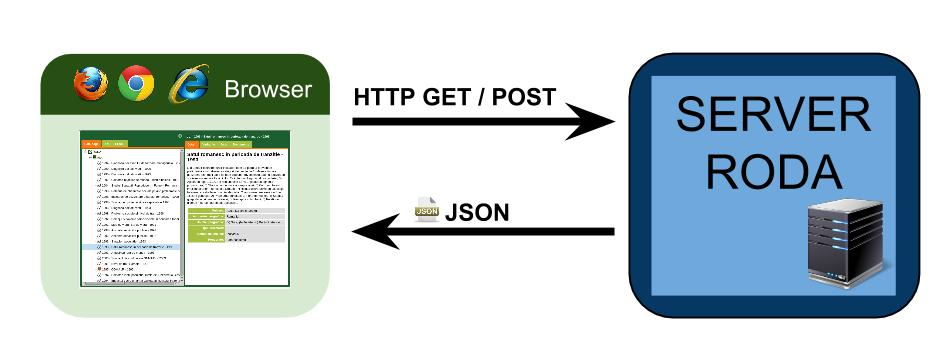
\includegraphics[width=9cm]{img/db-server}
\par\end{centering}
\caption{Modul simplificat de comunicare intre databrowser si server}
\end{figure}

\section{Controller-e JSON - server-side}

Controller-ele care stau la baza componentei Data Browser a aplicatiei utilizeaza servicii care, la randul lor, refera anumite clase speciale din domeniu. 
Aceste clase extind o clasa de baza (\emph{JsonInfo}), ce contine atributele comune ale claselor utilizate pentru obtinerea rezultatelor in format JSON. 
Pe langa acestea, atributul \emph{type} al clasei permite distinctia intre obiectele de diferite tipuri ce apar in ierarhii. 
Astfel, vom avea elemente al caror tip este M (nod principal, radacina in cazul ierarhiilor), C (catalog), S (serie), St (studiu), Sts (studiu ce provine dintr-o serie), Y (an).  
Subclasele lui \emph{JsonInfo} structureaza informatia necesara in rezultatul controller-elor, furnizand metode statice de generare a colectiilor corespunzatoare sau a obiectelor identificate cu ajutorul valorii cheii primare sau a altor campuri (de exemplu, valoarea anului pentru ierarhia de ani si studii). Cu ajutorul acestor metode, clasele ce extind \emph{JsonInfo} permit obtinerea de informatii complexe, care vizeaza mai multe clase ale domeniului de baza al aplicatiei.
Transformarea colectiilor sau obiectelor in format JSON s-a efectuat cu ajutorul bibliotecii \emph{Flexjson} (\url{http://flexjson.sourceforge.net/}) care permite serializarea, respectiv deserializarea obiectelor Java in si din JSON.  

Ierarhia de clase ce deriva din \emph{JsonInfo} cuprinde urmatoarele clase:
\begin{itemize}
\item
\emph{CatalogTree} - genereaza arborescenta de cataloage, pornind de la un nod principal (M), urmat de cataloagele radacina (care nu au un catalog parinte). La nivelul fiecarui catalog este indicat tipul acestuia (C sau S), iar la nivelul fiecarui studiu este indicat tipul acestuia (St sau Sts). Un studiu poate apartine si unui alt catalog, de tip serie; astfel, in cazul unui studiu de tip Sts este indicat si codul seriei care il contine. In frunzele arborelui se afla studiile.
\item
\emph{StudiesByCatalog} - prezinta studiile din cadrul fiecarui catalog din baza de date. La nivelul fiecarui catalog este indicat numarul studiilor sale, iar la nivelul fiecarui studiu este indicat tipul acestuia (St sau Sts). 
\item
\emph{StudiesBySeries} - prezinta studiile din seriile din baza de date; pentru fiecare serie, este specificat si numarul studiilor din cadrul sau. 
\item
\emph{StudiesByTopic} - prezinta studiile corespunzatoare fiecarui topic.
\item
\emph{StudiesByYear} - prezinta studiile corespunzatoare fiecarui an in care s-au realizat studii, precum si numarul acestora. La nivelul fiecarui studiu este specificat tipul (St sau Sts).
\item
\emph{StudyInfo} - genereaza informatii complete despre studiile din baza de date, incluzand variabilele, persoanele, organizatiile, fisierele si cuvintele cheie asociate) 
\item
\emph{YearsTree} - genereaza ierarhia corespunzatoare anilor, pornind de la un nod principal (M), ai carui fii (de tip Y) corespund anilor de realizare a studiilor din baza de date. La nivelul fiecarui studiu este indicat tipul acestuia (St sau Sts) 
\end{itemize}

Fiecarei clase de mai sus ii corespunde un controller in pachetul 'ro.roda.web' (\emph{<NumeClasa>Controller}), ce utilizeaza un serviciu asociat in pachetul 'ro.roda.service' (\emph{<NumeClasa>Service}).

\section{DataBrowser API}

In acest moment, interfata serverului pentru DataBrowser contine urmatoarele
apeluri si rezultate:

\subsection{CatalogTree}

Returneaza o lista a tuturor cataloagelor generale din sistem impreuna
cu studiile asociate acestora. Structura este arborescenta, elementul
de container se numeste \textquotedbl{}data\textquotedbl{}

\begin{figure}[H]
\begin{centering}
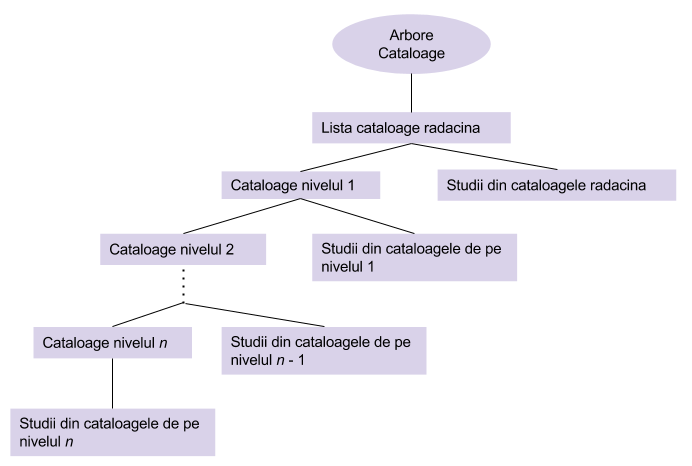
\includegraphics[width=9cm]{img/catalogtree}
\par\end{centering}
\caption{Etapele de procesare ale serverului necesare pentru returnarea raspunsului}
\end{figure}

\begin{itemize}
\item \textbf{name} - Numele catalogului 
\item \textbf{type} - Tipul catalogului 

\begin{itemize}
\item \textbf{M} - Master catalog, catalogul principal, radacina pentru
celelalte cataloage publice 
\item \textbf{C} - Catalog normal 
\item \textbf{S} - Serie (studii grupate de catre executanti dupa orice
criteriu) 
\end{itemize}
\item \textbf{indice} - indexul numeric unic al catalogului din baza de
date 
\item \textbf{data} - continutul catalogului. Acesta poate cuprinde alte
cataloage (cu aceeasi structura ca mai sus), serii sau studii 

\begin{itemize}
\item \textbf{an} - Anul in care a fost finalizat studiul 
\item \textbf{description} - rezumatul studiului 
\item \textbf{geographicUnit} - Unitatea geografica pe care se bazeaza realizarea
studiului 
\item \textbf{indice} - id-ul unic din baza de date al studiului 
\item \textbf{name} - titlul studiului 
\item \textbf{researchInstrument }- Tipul cercetarii 
\item \textbf{seriesId} - in cazul in care studiul este membru al unei serii,
aici se inregistreaza, pentru referinta, id-ul unic din baza de date
al seriei respective 
\item \textbf{type} - tipul studiului, care determina mudul de afisare in
panoul de detalii 

\begin{itemize}
\item \textbf{St} - studiu izolat 
\item \textbf{Sts} - membru al unei serii weighting - metoda de ponderare
folosita
\end{itemize}
\end{itemize}
\end{itemize}

\subsection{YearTree}

Returneaza o lista a tuturor anilor din sistem care au studii asociate
acestora, impreuna cu studiile corespunzatoare. Structura este arborescenta,
elementul de container se numeste \textquotedbl{}data\textquotedbl{}.
Structura este deschisa de un nod unic principal.

\begin{figure}[H]
\begin{centering}
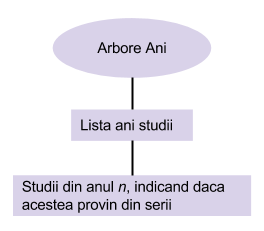
\includegraphics[width=4cm]{img/yearstree}
\par\end{centering}
\caption{Etapele de procesare ale serverului}
\end{figure}

\paragraph{Nodul principal}
\begin{itemize}
\item \textbf{name} - Numele nodului principal (doar in cazul nodului principal) 
\item \textbf{type} - Tipul nodului 
\item \textbf{M }- Master, nodul principal, radacina pentru nodurile pe
ani 
\item \textbf{data} - continutul nodului (lista nearborescenta de ani)
\end{itemize}

\paragraph{Nod de tip an}
\begin{itemize}
\item \textbf{name} - Numele nodului de tip an 
\item \textbf{an} - Anul nodului curent 
\item \textbf{type} - Y 
\item \textbf{data} - continutul nodului (lista nearborescenta de studii) 

\begin{itemize}
\item \textbf{an} - Anul in care a fost finalizat studiul 
\item \textbf{description} - rezumatul studiului 
\item \textbf{geographicUnit} - Unitatea geografica pe care se bazeaza realizarea
studiului 
\item \textbf{indice} - id-ul unic din baza de date al studiului 
\item \textbf{name} - titlul studiului 
\item \textbf{researchInstrument} - Tipul cercetarii 
\item \textbf{seriesId} - in cazul in care studiul este membru al unei serii,
aici se inregistreaza, pentru referinta, id-ul unic din baza de date
al seriei respective 
\item \textbf{type} - tipul studiului, care determina mudul de afisare in
panoul de detalii 

\begin{itemize}
\item \textbf{St} - studiu izolat 
\item \textbf{Sts} - membru al unei serii 
\end{itemize}
\item \textbf{weighting} - metoda de ponderare folosita 
\end{itemize}
\end{itemize}

\subsection{StudyInfo}

Returneaza principalele componente ale structurii asociate unui studiu

\begin{figure}[H]
\begin{centering}
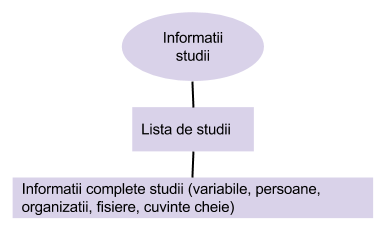
\includegraphics[width=5cm]{img/studyinfo}
\par\end{centering}
\caption{Etapele de procesare ale serverului necesare pentru returnarea raspunsului}
\end{figure}

\begin{itemize}
\item \textbf{an} - Anul in care a fost finalizat studiul 
\item \textbf{description} - rezumatul studiului 
\item \textbf{geographicUnit} - Unitatea geografica pe care se bazeaza realizarea
studiului 
\item \textbf{indice} - id-ul unic din baza de date al studiului 
\item \textbf{name} - titlul studiului 
\item \textbf{researchInstrument} - Tipul cercetarii 
\item \textbf{seriesId} - in cazul in care studiul este membru al unei serii,
aici se inregistreaza, pentru referinta, id-ul unic din baza de date
al seriei respective 
\item \textbf{type} - tipul studiului, care determina mudul de afisare in
panoul de detalii 

\begin{itemize}
\item \textbf{St} - studiu izolat 
\item \textbf{Sts} - membru al unei serii 
\end{itemize}
\item \textbf{weighting} - metoda de ponderare folosita 
\item \textbf{research\_instrument} - Tipul de cercetare 
\item \textbf{unit\_analysis} - Unitatea de analiza a studiului 
\item \textbf{universe} - universul studiului 
\item \textbf{keywords} - Cuvintele cheie ale studiului 
\item \textbf{orgs} - Organizatii asociate studiului 
\item \textbf{persons} - Persoane asociate studiului 
\item \textbf{variables} - Colectie de variabile 

\begin{itemize}
\item \textbf{nrfreq} - Numarul frecventelor calculate pentru variabila
curenta 
\item \textbf{indice} - Indexul unic al variabilei in baza de date 
\item \textbf{label }- Eticheta variabilei 
\item \textbf{name} - Numele variabilei 
\end{itemize}
\end{itemize}

\subsection{StudiesbyCatalog}

Returneaza un nod de tip catalog impreuna cu toate studiile care fac
parte din acel catalog, in lista aplatizata (daca exista subcataloage
acestea nu sunt returnate dar studiile asociate lor, da).

\begin{figure}[H]
\begin{centering}
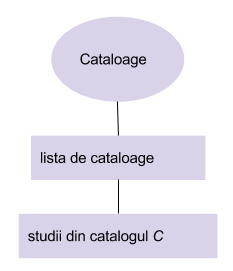
\includegraphics[width=4cm]{img/studiesbycatalog}
\par\end{centering}
\caption{Etapele de procesare ale serverului necesare pentru returnarea raspunsului}
\end{figure}

\begin{itemize}
\item \textbf{name} - Numele catalogului 
\item \textbf{nrstudies} - Numarul de studii 
\item \textbf{indice} - indexul numeric unic al catalogului din baza de
date 
\item \textbf{data} - continutul catalogului. Acesta cuprinde doar studii,
indiferent de structura arborescenta a subcataloagelor.

\begin{itemize}
\item \textbf{an} - Anul in care a fost finalizat studiul 
\item \textbf{description} - rezumatul studiului 
\item \textbf{geographicUnit} - Unitatea geografica pe care se bazeaza realizarea
studiului 
\item \textbf{indice} - id-ul unic din baza de date al studiului 
\item \textbf{name} - titlul studiului 
\item \textbf{researchInstrument} - Tipul cercetarii 
\item \textbf{seriesId} - in cazul in care studiul este membru al unei serii,
aici se inregistreaza, pentru referinta, id-ul unic din baza de date
al seriei respective 
\item \textbf{type} - tipul studiului, care determina modul de afisare in
panoul de detalii 

\begin{itemize}
\item \textbf{St} - studiu izolat 
\item \textbf{Sts }- membru al unei serii 
\end{itemize}
\item \textbf{weighting} - metoda de ponderare folosita 
\end{itemize}
\end{itemize}

\subsection{StudiesbySeries}

Returneaza un nod de tip serie impreuna cu toate studiile care fac
parte din aceasta

\begin{figure}[H]
\begin{centering}
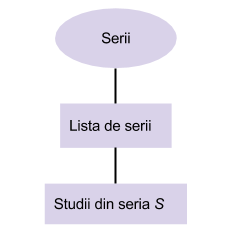
\includegraphics[width=4cm]{img/series}
\par\end{centering}
\caption{Etapele de procesare ale serverului necesare pentru returnarea raspunsului}
\end{figure}

\begin{itemize}
\item \textbf{description} - rezumatul seriei 
\item \textbf{geographicUnit} - Unitatea geografica pe care se bazeaza realizarea
seriei 
\item \textbf{indice} - id-ul unic din baza de date al seriei 
\item \textbf{name} - titlul seriei 
\item \textbf{researchInstrument} - Tipul cercetarii 
\item \textbf{weighting} - metoda de ponderare folosita, daca este comuna 
\item \textbf{research\_instrument} - Tipul de cercetare 
\item \textbf{unit\_analysis} - Unitatea de analiza a seriei 
\item \textbf{universe} - universul seriei 
\item \textbf{keywords} - Cuvintele cheie ale seriei 
\item \textbf{orgs }- Organizatii asociate seriei 
\item \textbf{persons} - Persoane asociate seriei 
\item \textbf{data} - continutul seriei, lista de studii 

\begin{itemize}
\item \textbf{an} - Anul in care a fost finalizat studiul 
\item \textbf{description} - rezumatul studiului 
\item \textbf{geographicUnit} - Unitatea geografica pe care se bazeaza realizarea
studiului 
\item \textbf{indice} - id-ul unic din baza de date al studiului 
\item \textbf{name} - titlul studiului 
\item \textbf{researchInstrument} - Tipul cercetarii 
\item \textbf{seriesId} - in cazul in care studiul este membru al unei serii,
aici se inregistreaza, pentru referinta, id-ul unic din baza de date
al seriei respective 
\item \textbf{type} - tipul studiului, care determina modul de afisare in
panoul de detalii 

\begin{itemize}
\item \textbf{Sts} - membru al unei serii 
\end{itemize}
\item \textbf{weighting} - metoda de ponderare folosita 
\end{itemize}
\end{itemize}

\subsection{StudiesbyYear}

Lista tuturor studiilor din acelasi an.

Returneaza un nod principal de tip an impreuna cu toate studiile asociate
acestuia:

\begin{figure}[H]
\begin{centering}
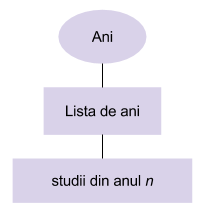
\includegraphics[width=4cm]{img/studiesbyyear}
\par\end{centering}
\caption{Etapele de procesare ale serverului necesare pentru returnarea raspunsului}
\end{figure}

\begin{itemize}
\item \textbf{name} - Numele nodului de tip an 
\item \textbf{an} - Anul nodului curent 
\item \textbf{type} - Y 
\item \textbf{data} - continutul nodului (lista nearborescenta de studii) 

\begin{itemize}
\item \textbf{an} - Anul in care a fost finalizat studiul 
\item \textbf{description} - rezumatul studiului 
\item \textbf{geographicUnit} - Unitatea geografica pe care se bazeaza realizarea
studiului 
\item \textbf{indice} - id-ul unic din baza de date al studiului name -
titlul studiului 
\item \textbf{researchInstrument} - Tipul cercetarii 
\item \textbf{seriesId} - in cazul in care studiul este membru al unei serii,
aici se inregistreaza, pentru referinta, id-ul unic din baza de date
al seriei respective 
\item \textbf{type} - tipul studiului, care determina modul de afisare in
panoul de detalii 

\begin{itemize}
\item \textbf{St} - studiu izolat 
\item \textbf{Sts} - membru al unei serii 
\end{itemize}
\item \textbf{weighting} - metoda de ponderare folosita
\end{itemize}
\end{itemize}

\section{Interfata}

Interfata DataBrowser-ului este compusa din doua zone principale,
zona de index si zona de detaliu. Zona de index contine mai multe
ecrane care afiseaza studiile aflate in baza de date in functie de
diferite criterii de grupare. Zona de index este construita pentru
a afisa diferite modalitati de trecere in revista a tuturor studiilor
din baza de date. In functie de necesitati, se pot adauga noi ecrane
care sa permita noi modalitati de grupare sau filtrare. Zona de detaliu
contine diferite tipuri de ecrane care afiseaza detalii despre elementul
selectat in zona de index. 

\begin{figure}[H]
\begin{centering}
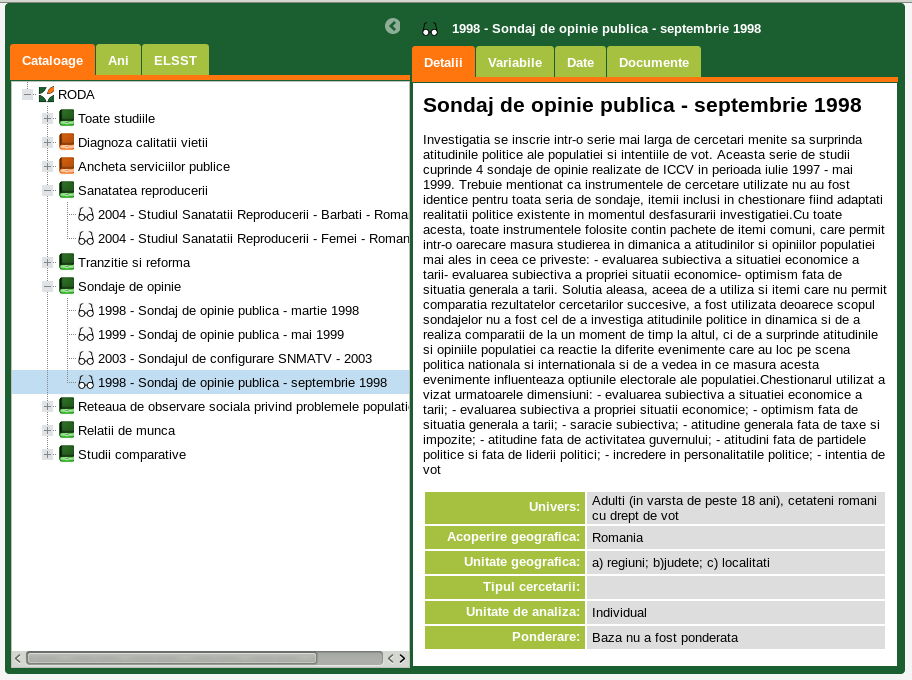
\includegraphics[width=11cm]{screenshots/databrowser-general}
\par\end{centering}
\caption{Databrowser}
\end{figure}

\subsection{Ecranele din zona de index}

\subsubsection{Cataloage}

Ecranul ``Cataloage'' afiseaza o structura arborescenta de cataloage,
serii si studii. Cataloagele sunt elemente arbitrare de grupare propuse
de RODA pentru gruparea studiilor. Cataloagele pot fi incluse in alte
cataloage. Un studiu poate fi membru in mai multe cataloage si in
acest caz el va aparea in toate. 

Un caz particular al cataloagelor sunt seriile. Seriile reprezinta
grupari ne-arbitrare de studii, alaturate conform unui criteriu important,
cum ar fi tematica lor. 

\begin{figure}[H]
\begin{centering}
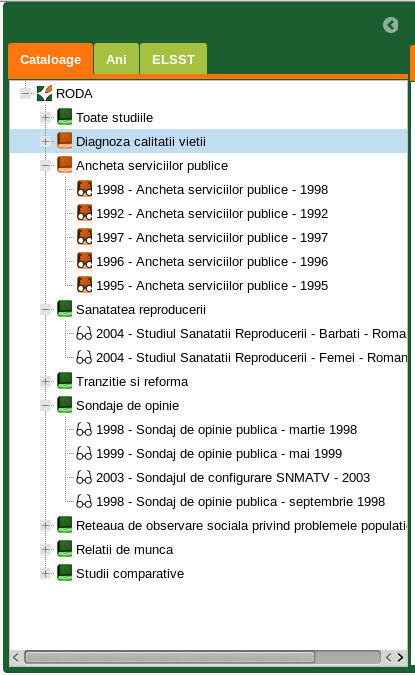
\includegraphics[width=6cm]{screenshots/left-panel-cataloage}
\par\end{centering}

\caption{Ecranul ``Cataloage''}
\end{figure}

\subsubsection{Ani}

Ecranul ``Ani'' afiseaza o structura arborescenta in care studiile
sunt grupate dupa ani. Studiile care sunt membre in serii sunt evidentiate.
Seriile ca elemente de sine statatoare nu pot aparea aici pentru ca
studiile din aceeasi serie pot fi (si de obicei sunt) finalizate in
ani diferiti. 

\begin{figure}[H]
\begin{centering}
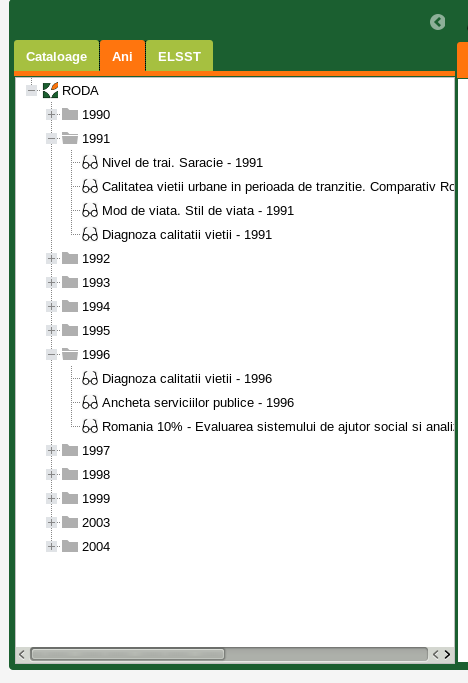
\includegraphics[width=6cm]{screenshots/left-panel-ani}
\par\end{centering}
\caption{Ecranul ``Ani''}
\end{figure}

\subsection{Ecrane din zona de detaliu}
\subsubsection{Catalog}

Ecranul pentru vizualizarea catalogului afiseaza toate studiile din
catalogul selectat. Acest ecran apare doar cand in zona de index se
selecteaza un element de tip catalog. Acesta contine elemente care
permit cautarea locala (in catalogul curent) precum si elemente de
paginare. Ecranul pentru vizualizarea catalogului poate avea trei
densitati de informatie diferite. In cele ce urmeaza vor fi prezentate
cele trei ecrane asa cum sunt ele acum. Trebuie mentionat insa ca
elementele din cele trei ecrane se pot modifica in functie de evaluarea
utilizabilitatii interfetei.

\begin{figure}[H]
\begin{centering}
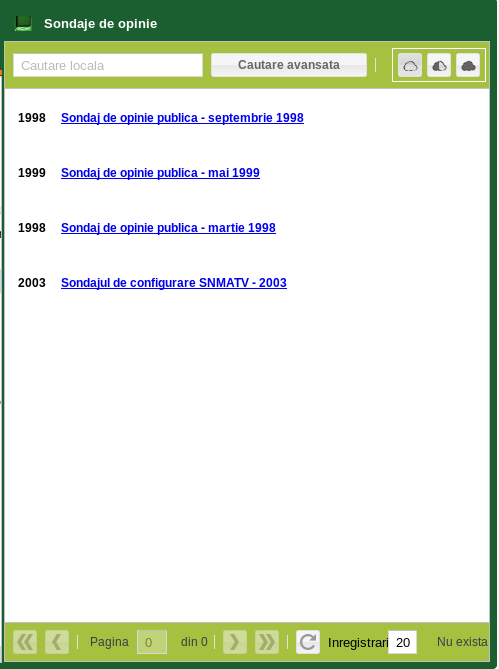
\includegraphics[width=6cm]{screenshots/details-panel-catalog-simple}
\par\end{centering}
\caption{Ecranul de tip Catalog - densitate de informatie mica}
\end{figure}

Ecranul cu densitate de informatie mica afiseaza anul si titlul studiului.
Titlul studiului este in acelasi timp si un link. La accesarea acestuia,
ecranul catalogului va fi inlocuit de ecranul care prezinta studiul
respectiv. 

\begin{figure}[H]
\begin{centering}
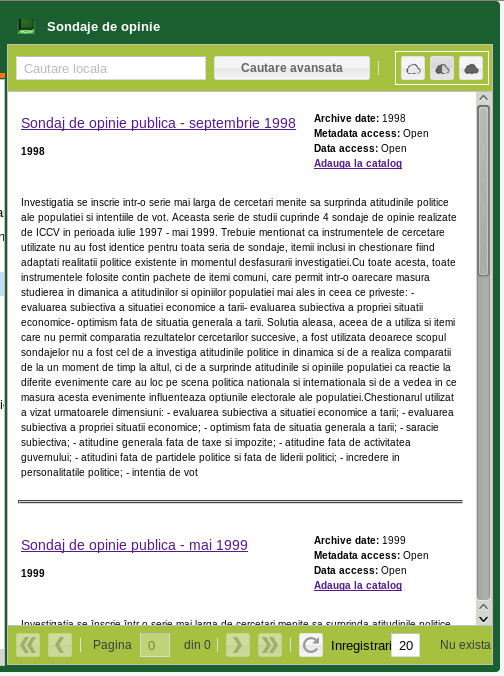
\includegraphics[width=6cm]{screenshots/details-panel-catalog-medium}
\par\end{centering}
\caption{Ecranul de tip Catalog - densitate de informatie medie}
\end{figure}

Ecranul cu densitate de informatie medie afiseaza titlul studiilor,
anul, informatii despre accesibilitatea metadatelor si datelor si
descrierea acestora. Pentru utilizatorii inregistrati va exista si
optiunea de a adauga studiile la un catalog personal. 

\begin{figure}[H]
\begin{centering}
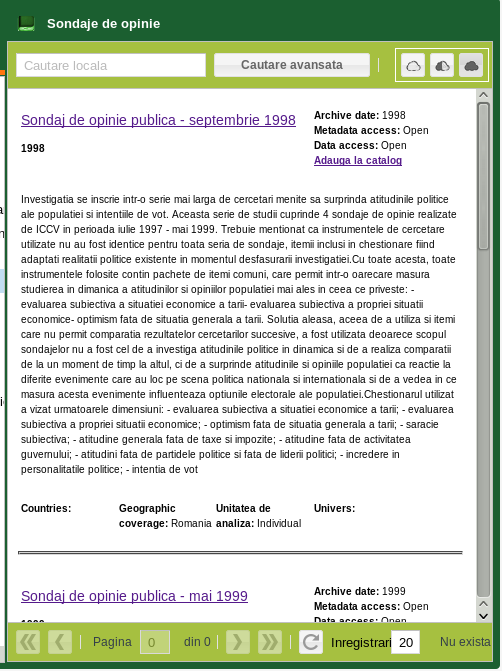
\includegraphics[width=6cm]{screenshots/details-panel-catalog-large}
\par\end{centering}
\caption{Ecranul de tip catalog - densitate de informatie mare}
\end{figure}

Ecranul cu densitate mare de informatie afiseaza toate informatiile
pe care le afiseaza ecranul cu densitate medie la care se adauga si
informatiile de localizare, unitatea de analiza, precum si alte elemente
tehnice care sunt dependente de tipul studiului. 

\subsection{Ani}

Ecranul pentru vizualizarea unui an afiseaza toate studiile din acel
an. Acest ecran apare doar cand in zona de index se selecteaza un
element de tip an. Ecranul contine elemente care permit cautarea locala
(in catalogul curent) precum si elemente de paginare. Ecranul pentru
vizualizarea anului poate avea trei densitati de informatie diferite. 

\begin{figure}[H]
\begin{centering}
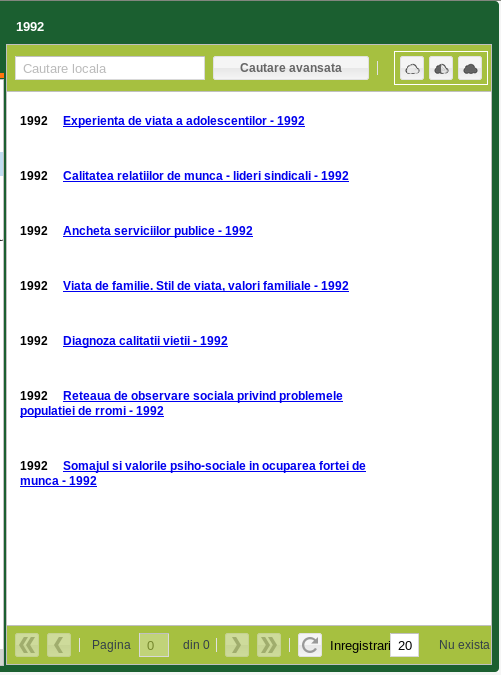
\includegraphics[width=6cm]{screenshots/details-panel-an-simple}
\par\end{centering}
\caption{Ecranul de tip an - densitate de informatie mica}
\end{figure}

Ecranul cu densitate de informatie mica afiseaza anul si titlul studiului.
Titlul studiului este in acelasi timp si un link. La accesarea acestuia,
ecranul catalogului va fi inlocuit de ecranul care prezinta studiul
respectiv. 

\begin{figure}[H]
\begin{centering}
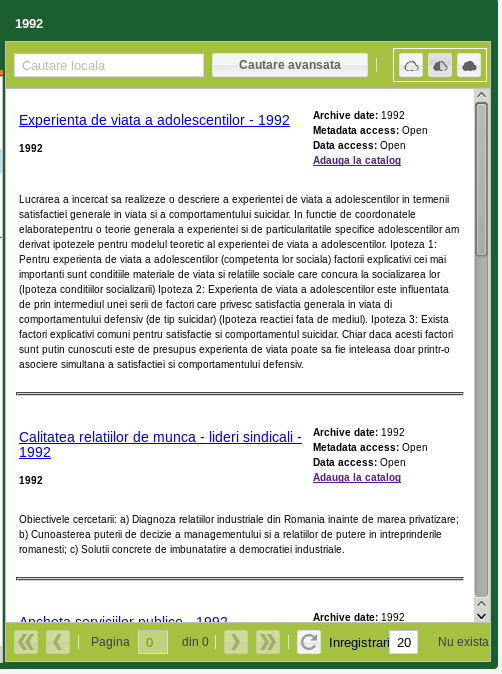
\includegraphics[width=6cm]{screenshots/details-panel-an-medium}
\par\end{centering}
\caption{Ecranul de tip an - densitate de informatie medie}
\end{figure}

Ecranul cu densitate de informatie medie afiseaza titlul studiilor,
anul, informatii despre accesibilitatea metadatelor si datelor si
descrierea acestora. Pentru utilizatorii inregistrati va exista si
optiunea de a adauga studiile la un catalog personal. 

\begin{figure}[H]
\begin{centering}
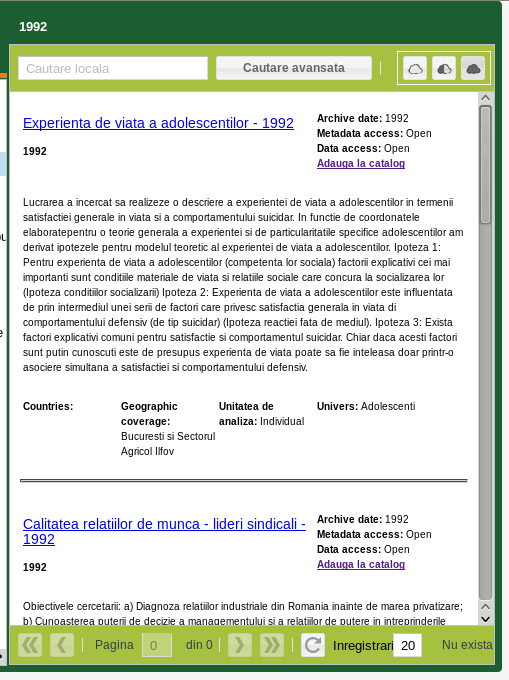
\includegraphics[width=6cm]{screenshots/details-panel-an-large}
\par\end{centering}
\caption{Ecranul de tip an - densitate de informatie mare}
\end{figure}

\subsection{Studiu}

Ecranul pentru afisarea unui studiu contine in acest moment patru
sub-ecrane. Acestea sunt configurate pentru studii de tip chestionar,
acestea fiind cele disponibile pentru date de testare. Pe masura ce
apar alte tipuri de studii, cu alte tipuri de metadate si date, structura
ecranului de studii se va modifica. 

\begin{figure}[H]
\begin{centering}
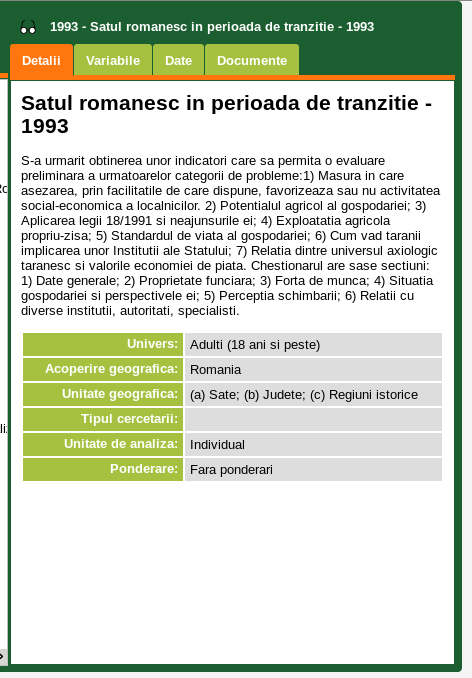
\includegraphics{screenshots/details-panel-study-detalii}
\par\end{centering}
\caption{Ecranul studiu, subecranul ``Detalii''}
\end{figure}

Subecranul ``detalii `` afiseaza titlul, descrierea si celelalte
metadate asociate studiului respectiv. In functie de metadatele disponibile
acest ecran poate contine diferite tipuri de informatii. Acest sub-ecran
va fi mentinut in toate ecranele care vor fi folosite pentru afisarea
diferitelor tipuri de studii.

\begin{figure}[H]
\begin{centering}
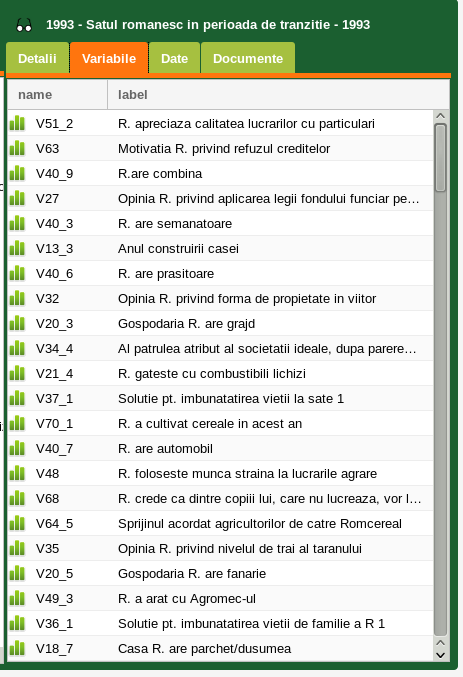
\includegraphics[width=6cm]{screenshots/details-panel-study-variabile}
\par\end{centering}
\caption{Ecranul studiu, subecranul ``Variabile''}
\end{figure}

Subecranul ``Variabile'', tipic pentru cercetarile sociologice bazate
pe chestionar, afiseaza un table cu toate variabilele (intrebarile)
din chestionar. Fiecare este afisata prin perechea nume - descriere,
la care se adauga si un element grafic care identifica prezenta valorilor
sintetice precalculate (ex: frecvente). Daca exista elementul grafic,
valorile precalculate pot fi vizualizate prin apasarea pe acesta.

\begin{figure}[H]
\begin{centering}
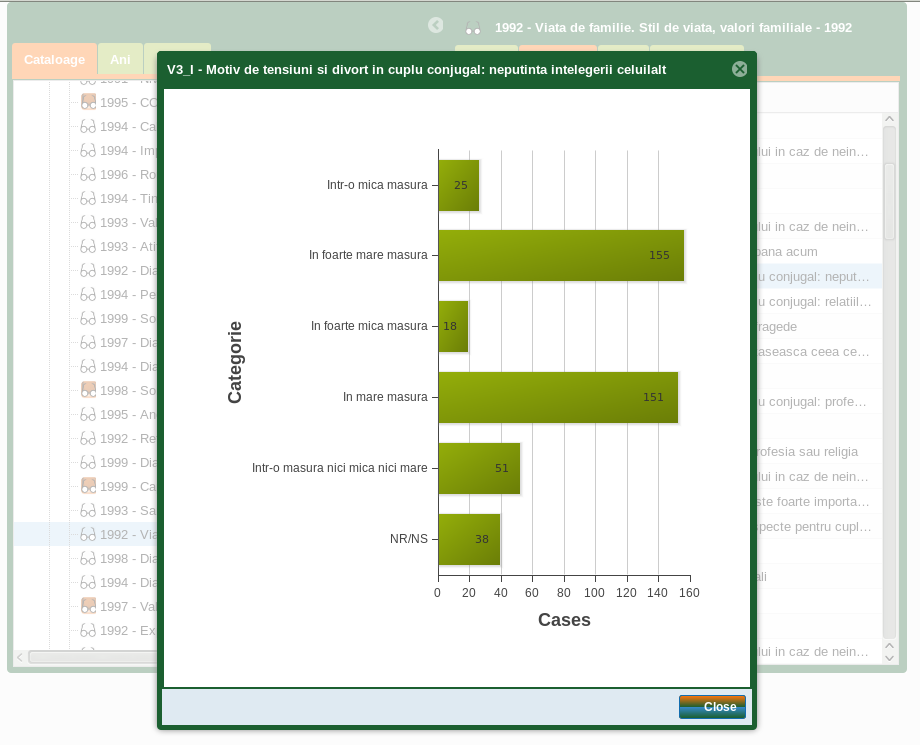
\includegraphics[width=11cm]{screenshots/details-panel-study-chart}
\par\end{centering}
\caption{Panoul care afiseaza valorile precalculate ale variabilelor}
\end{figure}

Panoul cu valori precalculate contine deocamdata graficul care afiseaza
numarul de raspunsuri la fiecare varianta pusa la dispozitie de catre
chestionar. Acest panou va fi extins pentru a contine si alte informatii,
inclusiv posibilitatea de a vedea in forma tabelara datele pe baza
carora este construit graficul. 

\begin{figure}[H]
\begin{centering}
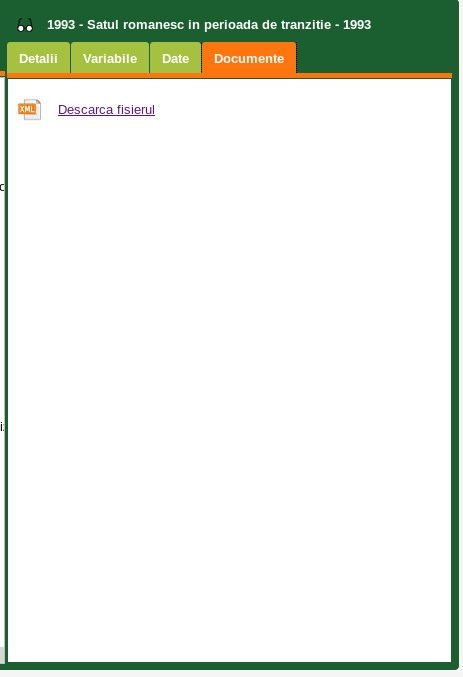
\includegraphics[width=6cm]{screenshots/details-panel-study-documente}
\par\end{centering}
\caption{Ecranul ``Studiu'', subecranul ``Documente''}
\end{figure}

Subecranul ``documente'' afiseaza si ofera spre descarcare toate
documentele atasate studiului curent. Acestea sunt dependente de modul
in care studiul a fost predat arhivei; in cazul de fata exista 
sursa acestuia in format DDI (XML), iar in alte situatii pot exista
mult mai multe.

\subsection{Serie}
Ecranul ``Serie'' afiseaza informatii despre o serie. O serie este
un grup de studii asemanatoare, executate, de exemplu, in ani diferiti,
pentru a urmari evolutia anumitor indicatori in timp. Astfel, o serie
reprezinta pe de-o parte un demers unitar, pe de alta parte o colectie
de studii. Pentru afisarea detaliilor unei serii se folosesc doua
subecrane, unul care afiseaza metadatele seriei (titlu, rezumat, precum
si alte metadate daca sunt disponibile) si un altul care afiseaza
lista studiilor care fac parte din acea serie. 

\begin{figure}[H]
\begin{centering}
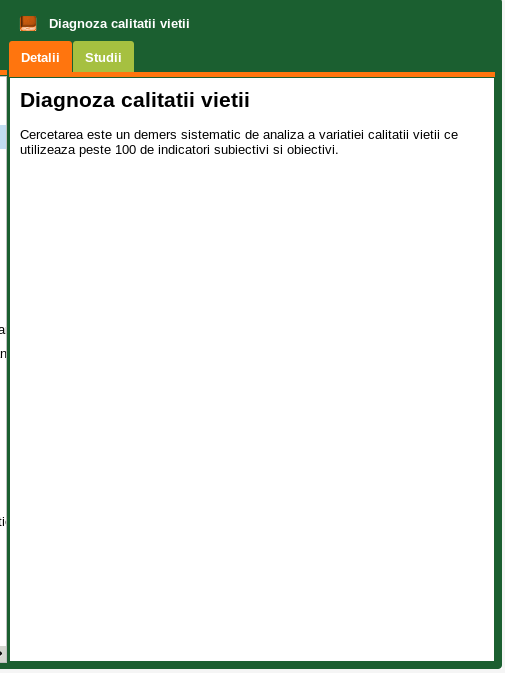
\includegraphics[width=6cm]{screenshots/details-panel-series-details}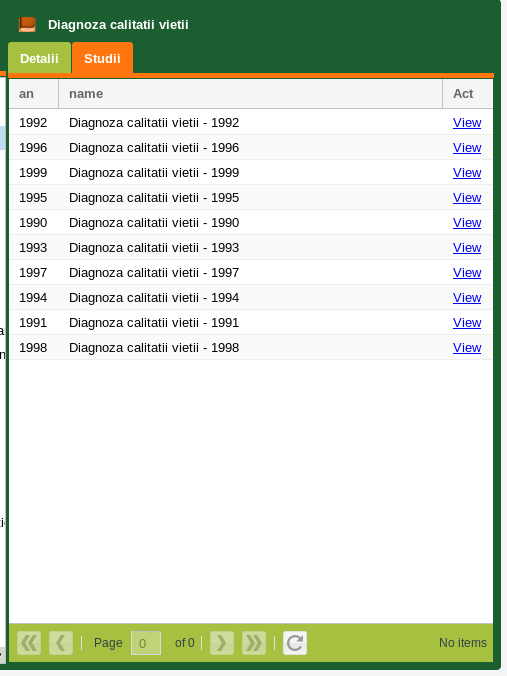
\includegraphics[width=6cm]{screenshots/details-panel-series-studies}
\par\end{centering}
\caption{Ecranul ``Serie'' subecranele ``Detalii'' si ``Studii''}
\end{figure}

\subsection{Membru al seriei}

Ecranul pentru un membru al unei serii este asemanator cu ecranul
unui studiu izolat. La el se adauga un subecran special care afiseaza
proprietatile seriei, asa cum sunt afisate si in sectiunea anterioara,
sub forma de meniu-acordeon.

\begin{figure}[H]
\begin{centering}
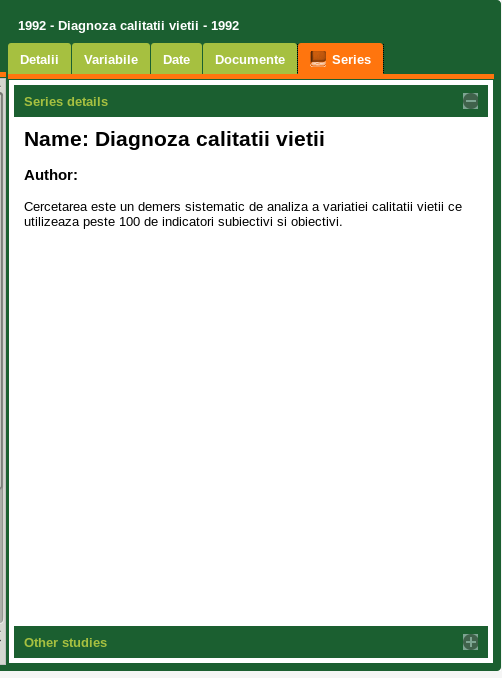
\includegraphics[width=6cm]{screenshots/details-panel-series-member-series-details}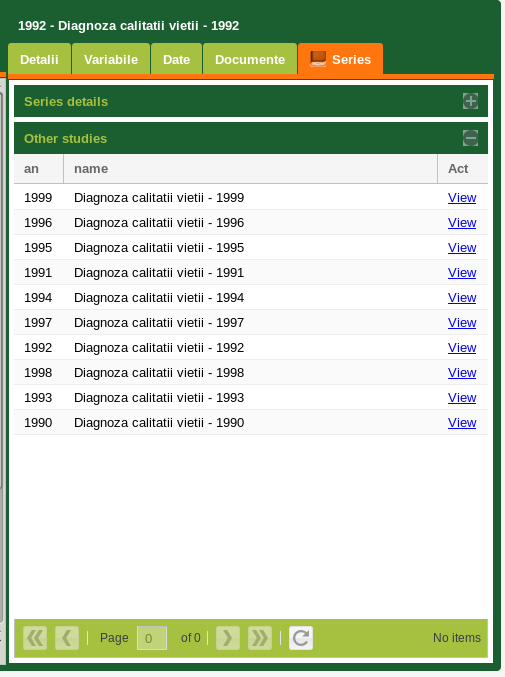
\includegraphics[width=6cm]{screenshots/details-panel-series-member-series-studies}
\par\end{centering}
\caption{Subecranul suplimentar pentru un studiu membru al unel serii}
\end{figure}


\chapter{Importarea datelor}
Datele initiale ale aplicatiei sunt importate chiar la pornirea serverului folosind un 'hook' al sistemului Spring MVC (ApplicationListener <ContextRefreshedEvent>).

Functionalitatile de importare a datelor sunt grupate intr-un singur serviciu (interfata si implementare) aflat in pachetul 'ro.roda.importer'.

Serviciul de import permite:
\begin{description}
\item
[Importarea datelor initiale ale aplicatiei] 

Aceste date cele ce vor fi folosite si in versiunea de productie a aplicatiei, precum: utilizatori si roluri, drepturi de acces standard, limbi, date geografice, thesaurus etc.
Se importa din mai multe formate:
\begin{itemize}
\item din format CSV (Comma-Separated Values). Se folosesc fie pachetul OpenCSV, fie API-ul oferit de driverul JDBC al Postgresql pentru a importa fisiere CSV).
\item din format SQL. Se foloseste fisierul 'import.sql', pe care componenta ORM (Hibernate) este configurata sa il importe la initializarea sa.
\item din thesaurus-ul ELSST. Se importa termenii si ulterior relatiile dintre ei din mai multe fisiere in format CSV, 
populandu-se mai multe tabele (cele din zona 'Topics' din schema bazei de date).
\item din formatul DDI-Codebook (Data Documentation Initiative, \url{http://www.ddialliance.org/Specification/DDI-Codebook/}).
\end{itemize}

\item
[Importarea datelor suplimentare / de testare pentru aplicatie.]

Aceste date sunt in format CSV. 
Sunt populate cu date mai multe tabele mai putin importante, care nu trebuie populate si in versiunea de productie, ci doar in cea de development si testare. 
\end{description}

Importer-ul din formatul DDI este realizat doar partial in aceasta faza a proiectului.
Se va folosi un pachet de clase Java derivat de catre JAXB de la definitia XML Schema a formatului DDI.
Aceasta componenta software va permite utilizarea integrala a datelor de tip legacy din arhiva electronica a RODA (50 studii sociale).


\chapter{Documentatie pentru dezvoltatorii aplicatiei} 
La specificarea in instructiunile de mai jos a sistemului de operare:
\begin{description} 
\item [MacOSX =] OS X version 10.8.3, 64 bit
\item [Ubuntu =] Ubuntu 12.04LTS, kernel 3.2.0-39-generic-pae, 32bit
\item [OpenSUSE = ] OpenSUSE 12.2
\item [Postgresql =] Postgresql 9.2.4
\item [Hibernate =] Hibernate 4.1.8
\item [DbWrench =] DbWrench 2.3.2
\item [STS =] Spring Tool Suite 3.2.0.RELEASE - based on Eclipse Juno 3.8.2
\item [Maven =] Maven 3
\item [JVM =] Java Virtual Machine (JVM) 1.6
\item [Jenkins =] Jenkins 1.515
\item [Solr =] Solr 4.2.1
\item [Sencha Architect =] Sencha Architect 2.2.2
\end{description}

\section{Instalare si configurare - servicii si software aditional}

\subsection{Instalarea pachetelor necesare}
\begin{description}
\item[Ubuntu:]
Se ruleaza urmatoarele comenzi, din shell:
\begin{lstlisting}[breaklines=true]
sudo apt-get install openjdk-6-jdk maven perl r-base r-base-dev pgadmin3
libtest-www-selenium-perl htmldoc graphviz rubygems postgresql-server

sudo gem install vmc
\end{lstlisting}

\item[OpenSUSE:]
% TODO ???
Maven se instaleaza manual sau dintr-un repository non-standard.

R se instaleaza manual sau dintr-un repository non-standard.

Test::WWW::Selenium se instaleaza din CPAN.

Se ruleaza urmatoarele comenzi, din shell:
\begin{lstlisting}[breaklines=true]
sudo zypper in openjdk-7-jdk perl pgadmin3 htmldoc graphviz ruby ruby-devel
rubygems postgresql

sudo gem install vmc
\end{lstlisting}

\item[MacOSX:]

Se ruleaza urmatoarele comenzi, din shell:
\begin{lstlisting}[breaklines=true]
sudo port install maven3 perl5 R pgadmin3 p5.12-test-www-selenium
htmldoc graphviz rb-rubygems postgresql92

sudo gem install vmc
\end{lstlisting}
\end{description}

\subsection{Postgresql}
\begin{description}
\item[MacOSX:]

Se instaleaza si ruleaza Postgres.app (descarcat de la \url{http://postgresapp.com} ).
Se bifeaza in meniu optiunea 'Automatically Start at Login'.

Se instaleaza MacPorts si toate dependentele necesare (instructiuni complete la:
\url{http://www.macports.org/install.php} ).

\item[orice alt sistem de operare:]

Se configureaza Postgresql ca server pe statia locala (preferabil, pornit
automat ca serviciu la bootare). 
Se configureaza in fisierele de configurare ale Postgresql drepturile
de acces ale clientilor la server, de ex. pentru a permite accesul prin
internet, nu doar de la statia locala / reteaua locala.
% TODO mai precis ???
\end{description}

\subsection{LaTeX}
O distributie LaTeX este necesara pentru generarea documentatiei:
\begin{description}
\item[Ubuntu:] 

\begin{lstlisting}[breaklines=true]
	sudo apt-get install texlive
\end{lstlisting}

\item[MacOSX:] 
MacTeX, instalata de la \url{http://tug.org/mactex/} 
\end{description}

\subsection{Maven si Java Virtual Machine (JVM)}
Se creeaza in directorul \emph{\$HOME} al utilizatorului un fisier numit
'.mavenrc' 
(ce contine setarile generale pentru Maven, in acest caz legate de memoria utilizata);
in fisier se scrie:
\begin{lstlisting}[breaklines=true]
	MAVEN_OPTS='-Xmx1024m -XX:MaxPermSize=256m'
	export MAVEN_OPTS
\end{lstlisting}

\label{java_version}
Se verifica instalarea Java (e necesar minim Java 1.6) si tipul de JVM
utilizat (32 sau 64 bit), in shell:
\begin{lstlisting}
	java -version
\end{lstlisting}

\subsection{rJava}
Se instaleaza rJava in R, cu urmatoarele comenzi in shell si apoi in shell-ul R
(se alege in timpul instalarii site-mirror-ul folosit, dintr-o fereastra;
se iese la final din shell-ul R cu Ctrl+D):
\begin{lstlisting}
	sudo R CMD javareconf
	R
	install.packages('rJava')
\end{lstlisting}

\subsection{DbWrench}
Se instaleaza DbWrench de pe site-ul producatorului:
\url{http://www.dbwrench.com}.

\section{Instalarea si configurarea IDE-ului si a proiectului}

\subsection{Instalare Spring Tool Suite (STS)}
Descarcati STS de pe pagina:
\url{http://www.springsource.org/downloads/sts-ggts},
facand click direct pe link-ul \emph{'Just take me to the download page'}.

Alegeti pentru descarcarea versiunea STS bazata pe Eclipse 3.8.2, extensia
fisierului de salvat fiind '.sh', iar arhitectura cea stabilita de versiunea
JVM (32 sau 64 bit, vezi \ref{java_version}); pe website, sectiunea respectiva
este cea intitulata:
\begin{verbatim}
	Milestone Version - 
	Spring Tool Suite 3.2.0.RELEASE - 
	based on Eclipse Juno 3.8.2
\end{verbatim}

Instalati STS din shell (fara 'sudo'), cu optiunile default (se poate
schimba eventual path-ul care este propus de wizard pentru instalarea STS,
path-ul default este \emph{\$HOME/springsource} ):
'Next' -> ... -> 'Finish'.

\subsection{Configurarea STS inainte de rulare}
In fisierul \emph{STS.ini} (in Ubuntu/OpenSUSE, acesta este in folder-ul
radacina al STS, ales la pasul anterior; in MacOS X, este in sub-folder-ul
'STS.app/Contents/MacOS/'), se modifica memoria maxima utilizabila de STS.

In \emph{STS.ini}, linia care incepe cu \emph{-Xmx} 
(memoria maxima utilizabila de STS) 
trebuie modificata astfel:
\begin{itemize} 
\item daca JVM este pe 64 biti:
\begin{lstlisting}
	-Xmx3072m
\end{lstlisting}
\item daca JVM este pe 32 biti:
\begin{lstlisting}
	-Xmx1536m
\end{lstlisting}
\end{itemize}

\subsection{Configurarea STS}

Porniti STS, eventual din linia de comanda, in folder-ul radacina al instalarii STS:
\begin{lstlisting}	
	./STS &
\end{lstlisting}

Din Dashboard (meniu Help -> Dashboard), click pe tab-ul 'Extensions'
(pozitionat stanga-jos, in Dashboard), bifati in lista si apoi instalati
(butonul 'Install', dreapta-jos) urmatoarele extensii:
\begin{itemize}
\item
Cloud Foundry Eclipse Integration
\item
Edgewall Trac
\end{itemize} 

Restartati STS.

Instalati in STS ultima versiune de Subclipse (cu suport pentru Subversion 1.7),
prin meniu 'Help' -> 'Install New Software':
\begin{itemize}
\item 
nume = Subclipse 1.8
\item
URL = \url{http://subclipse.tigris.org/update_1.8.x}
\end{itemize}

Selectati si instalati de la acest update-site ambele seturi de plugin-uri:
'Subclipse' si 'SVNKit'.

Restartati STS.

Configurati Subclipse pentru a utiliza SVNKIT:
\begin{enumerate}
\item 
click pe meniu 'Window' -> 'Preferences' -> alegere din lista 'Team' -> 'SVN'
(pe MacOSX: meniu 'Spring Tool Suite' -> 'Preferences' -> 'Team' -> 'SVN')
\item
la 'SVN Interface' (mai jos in pagina de optiuni aparuta) se alege Clientul
folosit:

'SVNKit (pure Java) SVNKit v1.7....'
\end{enumerate}

Instalati plugin-ul IDE pentru Perl, prin meniu Help -> Install
New Software:
\begin{itemize}
\item 
nume = Perl EPIC
\item
URL = \url{http://e-p-i-c.sf.net/updates/testing}
\end{itemize}

\subsection{Preluare proiecte din repository-ul Subversion}
In STS, adaugati un SVN repository (in perspectiva 'SVN Repository
Exploring'), 

URL = \url{svn://fisiere.dyndns.org/roda}

Faceti \emph{Checkout} din SVN repository (click-dreapta pe numele
proiectului, apoi 'Checkout') ale urmatoarelor directoare:
\begin{description}
\item [roda:] aplicatia web Java / Spring / Roo
\item [(OPTIONAL) dbwrench2-files:] fisierele dbWrench, SQL si scripturile asociate
\item [(OPTIONAL) RODA-Model:] modelul Perl
\end{description}

\begin{comment}
In STS, se face upgrade la Subversion 1.7 (pt. working copy) pentru fiecare din proiectele de mai sus: 
in perspectiva 'Spring', 
in view-ul 'Package Explorer' sau in view-ul 'Navigator', 
click-dreapta pe numele proiectului respectiv,
si apoi in meniul aparut:
'Team' -> 'Upgrade' -> 'OK'. 
Poate aparea un mesaj de eroare/warning, care indica
faptul ca working-copy local este deja conform versiunii 1.7 a SVN.
\end{comment}

\subsection{Configurare Task Repository}
In STS, in view-ul 'Task List', butonul 'Add Repository', de tipul 'Trac', 
iar in pasul urmator:
\begin{itemize}
\item 
Server URL:    \url{http://fisiere.dyndns.org:8888/roda}
\item
Debifare optiune 'Anonymous'
\item
Completare User si Parola (specifice)
\item
Bifare 'Save password'
\item
'Validate Settings'
\item
'Finish'
\end{itemize}

La ultimul pas, se adauga un Query legat de acest Task-Repository (de exemplu,
se completeaza doar un nume - precum 'ALL' - si se apasa 'Finish').

\subsection{Setari STS pentru Java si Spring}
In fereastra 'Preferences' a STS:
\begin{itemize}
\item
in Java -> Editor -> Save Actions, se bifeaza: 'Perform the selected actions on save' ; ' Format source code' (format all lines).
\item
in Java -> Code Style -> Formatter, se selecteaza profilul 'Eclipse [built-in]', se apasa 'Edit', in tab-ul 'Line Wrapping' , campul 'Maximum line width' se completeaza cu '120' (in loc de 80).
Se completeaza in partea de sus numele profilului: 'RODA' , se apasa 'OK'.
\item
(optional) in Java -> Appearance -> Members Sort Order, se bifeaza 'Sort member in same category by visibility'.
\item
(optional) in SpringSource -> Dashboard, se debifeaza 'Show Dashboard on Startup'.
\end{itemize}

\section{Configurarea locala a proiectului}

\subsection{Configurarea serverului Postgresql local}
Folosind pentru conectare in linia de comanda
\begin{lstlisting}
	psql -h localhost
\end{lstlisting}
se dau comenzile:
\begin{lstlisting}
	CREATE USER roda PASSWORD 'roda';
	CREATE DATABASE roda OWNER roda ENCODING 'UTF8';
\end{lstlisting}

\section{Instalarea si configurarea serverului Solr local}

Se instaleaza Solr in '/opt'.
Pentru configurare se foloseste schema din subfolder-ul
'examples'. 

\subsection{Compilarea pentru prima data a proiectului}

In linia de comanda, in folderul-radacina al proiectului 'roda':
\begin{lstlisting}
	mvn -e -X clean package
\end{lstlisting}

Toate pachetele necesare sunt descarcate atunci cand se face prima compilare - care poate dura mai mult.

In STS, se alege perspectiva 'Spring', 
apoi click-dreapta in view-ul 'Package
Explorer' pe numele proiectului ('roda'), 
apoi din meniul aparut:
'Maven' -> 'Update Project', 
apoi 'OK'.

% STS va deschide un view numit 'Roo shell' unde se pot da comenzi Roo referitoare la proiect.

\subsection{Configurarea Serverului Local (in STS)}
Se trage (drag-and-drop) proiectul 'roda' din view-ul 'Package Explorer' 
peste serverul local prezent in view-ul 'Servers' (VMware vFabric tc Server ...).

\subsection{Fisierele de configurare ale aplicatiei}
Toate detaliile necesare se regasesc in sectiunea
dedicata fisierelor de configurare din capitolul dedicat componentelor/arhitecturii aplicatiei: 
\ref{fisiere_configurare}.

Configurarile \emph{default} din aceste fisiere nu trebuie neaparat
schimbate, daca se urmeaza intocmai acest ghid de instalare/configurare.

\section{Rularea locala a proiectului}

De fiecare data, inainte de pornirea aplicatiei, trebuie sa fie pornit Solr ca un server standalone pe portul 8983, folosind Jetty.
% TODO ???

\subsection{Rularea din STS, pe Server Local}
Se (re-)porneste serverul de aplicatii local folosind butoanele din view-ul
'Servers'.

Daca portul local 8080 era liber (portul se poate edita dupa dublu-click pe
server, in lista din view-ul 'Servers'), aplicatia e disponibila la:

\url{http://localhost:8080/roda}

\subsection{Rularea din linia de comanda, pe un Server Local ad-hoc de tip
Tomcat}
Din linia de comanda, in folder-ul radacina al proiectului 'roda', cu comanda:
\begin{lstlisting}
	mvn tomcat:run
\end{lstlisting}
Daca portul local 8080 era liber (portul se poate schimba in 'pom.xml'),
aplicatia e disponibila la:

\url{http://localhost:8080/roda}

\subsection{Rularea automata a testelor web (Selenium)}
Din linia de comanda, in folder-ul radacina al proiectului 'roda', cu comanda:
\begin{lstlisting}
	mvn tomcat:run selenium:selenese
\end{lstlisting}

\begin{comment}

\section{Rularea proiectului din STS, pe CloudFoundry (NERECOMANDAT)}

\paragraph{!!! ATENTIE !!!} 
Accesul la acest cont/server este shared (e folosit
inclusiv de catre Jenkins), 
pot aparea suprapuneri nedorite intre variante diferite / dezvoltatori diferiti !!!

Se adauga in view-ul 'Servers' un nou server remote: click-dreapta -> 'New'
-> 'Server' -> vendor 'VMware' -> tip 'Cloud Foundry' -> 'Next'.

Se completeaza wizard-ul conform urmatorilor pasi:
\begin{itemize}
  \item 
Email: roda.devel@gmail.com
  \item 
Parola: RodaAdor
  \item 
'Validate Account'
  \item 
'Next'
  \item 
Se muta proiectul 'roda' din lista 'Available' in lista 'Configured'
  \item 
'Next'
  \item 
In fereastra 'Application details', se selecteaza 'Application Type' = 'Spring'
  \item 
'Next'
  \item 
'Deployed URL': roda.cloudfoundry.com
  \item 
'Memory Reservation': 2048 M
  \item 
'Next'
  \item 
Se bifeaza serviciul 'roda-postgres' (baza de date Postgresql) in lista
aparuta.
  \item 
'Finish'
\end{itemize}

Proiectul este disponibil online permanent la adresa:

\url{http://roda.cloudfoundry.com}

\end{comment}

\section{Integrarea continua a aplicatiei}
\subsection{Instalarea si configurarea Jenkins}

Lista plugin-urilor Jenkins ce trebuie instalate:
\begin{itemize}
\item 
Ant Plugin
\item
conditional-buildstep
\item
Credentials Plugin
\item
External Monitor Job Type Plugin
\item
Flexible Publish Plugin
\item
GitHub API Plugin
\item
GitHub plugin
\item
Javadoc Plugin
\item
Jenkins CVS Plug-in
\item
Jenkins Email Extension Plugin
\item
Jenkins GIT client plugin
\item
Jenkins GIT plugin
\item
Jenkins Mailer Plugin
\item
Jenkins SSH Slaves plugin
\item
Jenkins Subversion Plug-in
\item
Jenkins Translation Assistance plugin
\item
Jenkins VirtualBox Plugin
\item
Jenkins Workspace Cleanup Plugin
\item
LDAP Plugin
\item
Maven 2 Project Plugin
\item
pam-auth
\item
Run Condition Plugin
\item
SSH Credentials Plugin
\item
Token Macro Plugin
\end{itemize}

% TODO ???


\chapter{Servicii TIC destinate echipei proiectului}
\begin{description}

\item[File-Server] (AjaXplorer) - pentru rapoarte, manuale, standarde, documente read-only, date legacy etc.

\item[Serviciu de versionare a codului-sursa] (Subversion 1.7) , inclusiv
    notificari prin e-mail

\item[Bugtracking si project-management] (Trac), inclusiv notificari prin
    e-mail si integrare cu IDE (Spring Tool Suite)

\item[Backup] - pentru datele aferente celor 3 servicii enumerate mai sus

\item[Lista de e-mailuri] - pentru coordonarea echipei de dezvoltare

\item[Serviciu de integrare continua] (Jenkins) - pentru asamblarea si
    testarea aplicatiei dezvoltate, in mod continuu, cu notificari

\item[Serviciu de indexare/cautare] (Apache Solr) - utilizabil in
    conjunctie cu aplicatia dezvoltata

\item[Document-Management Server] (Alfresco Community Edition 4.2) -
    utilizabil in conjunctie cu aplicatia dezvoltata

\item[Database server] (Postgresql) - utilizat in conjunctie cu
    aplicatia dezvoltata

\item[Development \& production web application servers] (Apache Tomcat 7) -
    gazduiesc aplicatia dezvoltata

\item[Server web] (Apache) - in curs de configurare

\item[Servicii de tip Director] (LDAP 3) - in curs de configurare

\item[Servicii de autentificare federata] (Shibboleth / SAML2) - in curs de
configurare

\end{description}


\end{document}
